
\documentclass[11pt]{article}
\usepackage{amsmath,amssymb}
\usepackage{graphicx}
\usepackage{natbib}
\usepackage[parfill]{parskip}
\usepackage[margin=1in]{geometry}
\usepackage{pdflscape}
\title{Supplementary information for ``CLM5-PPE"}
\author{D. Kennedy}
\renewcommand{\thefigure}{S\arabic{figure}}
\begin{document}
\maketitle


\begin{landscape}
\begin{figure}[h]
\centering
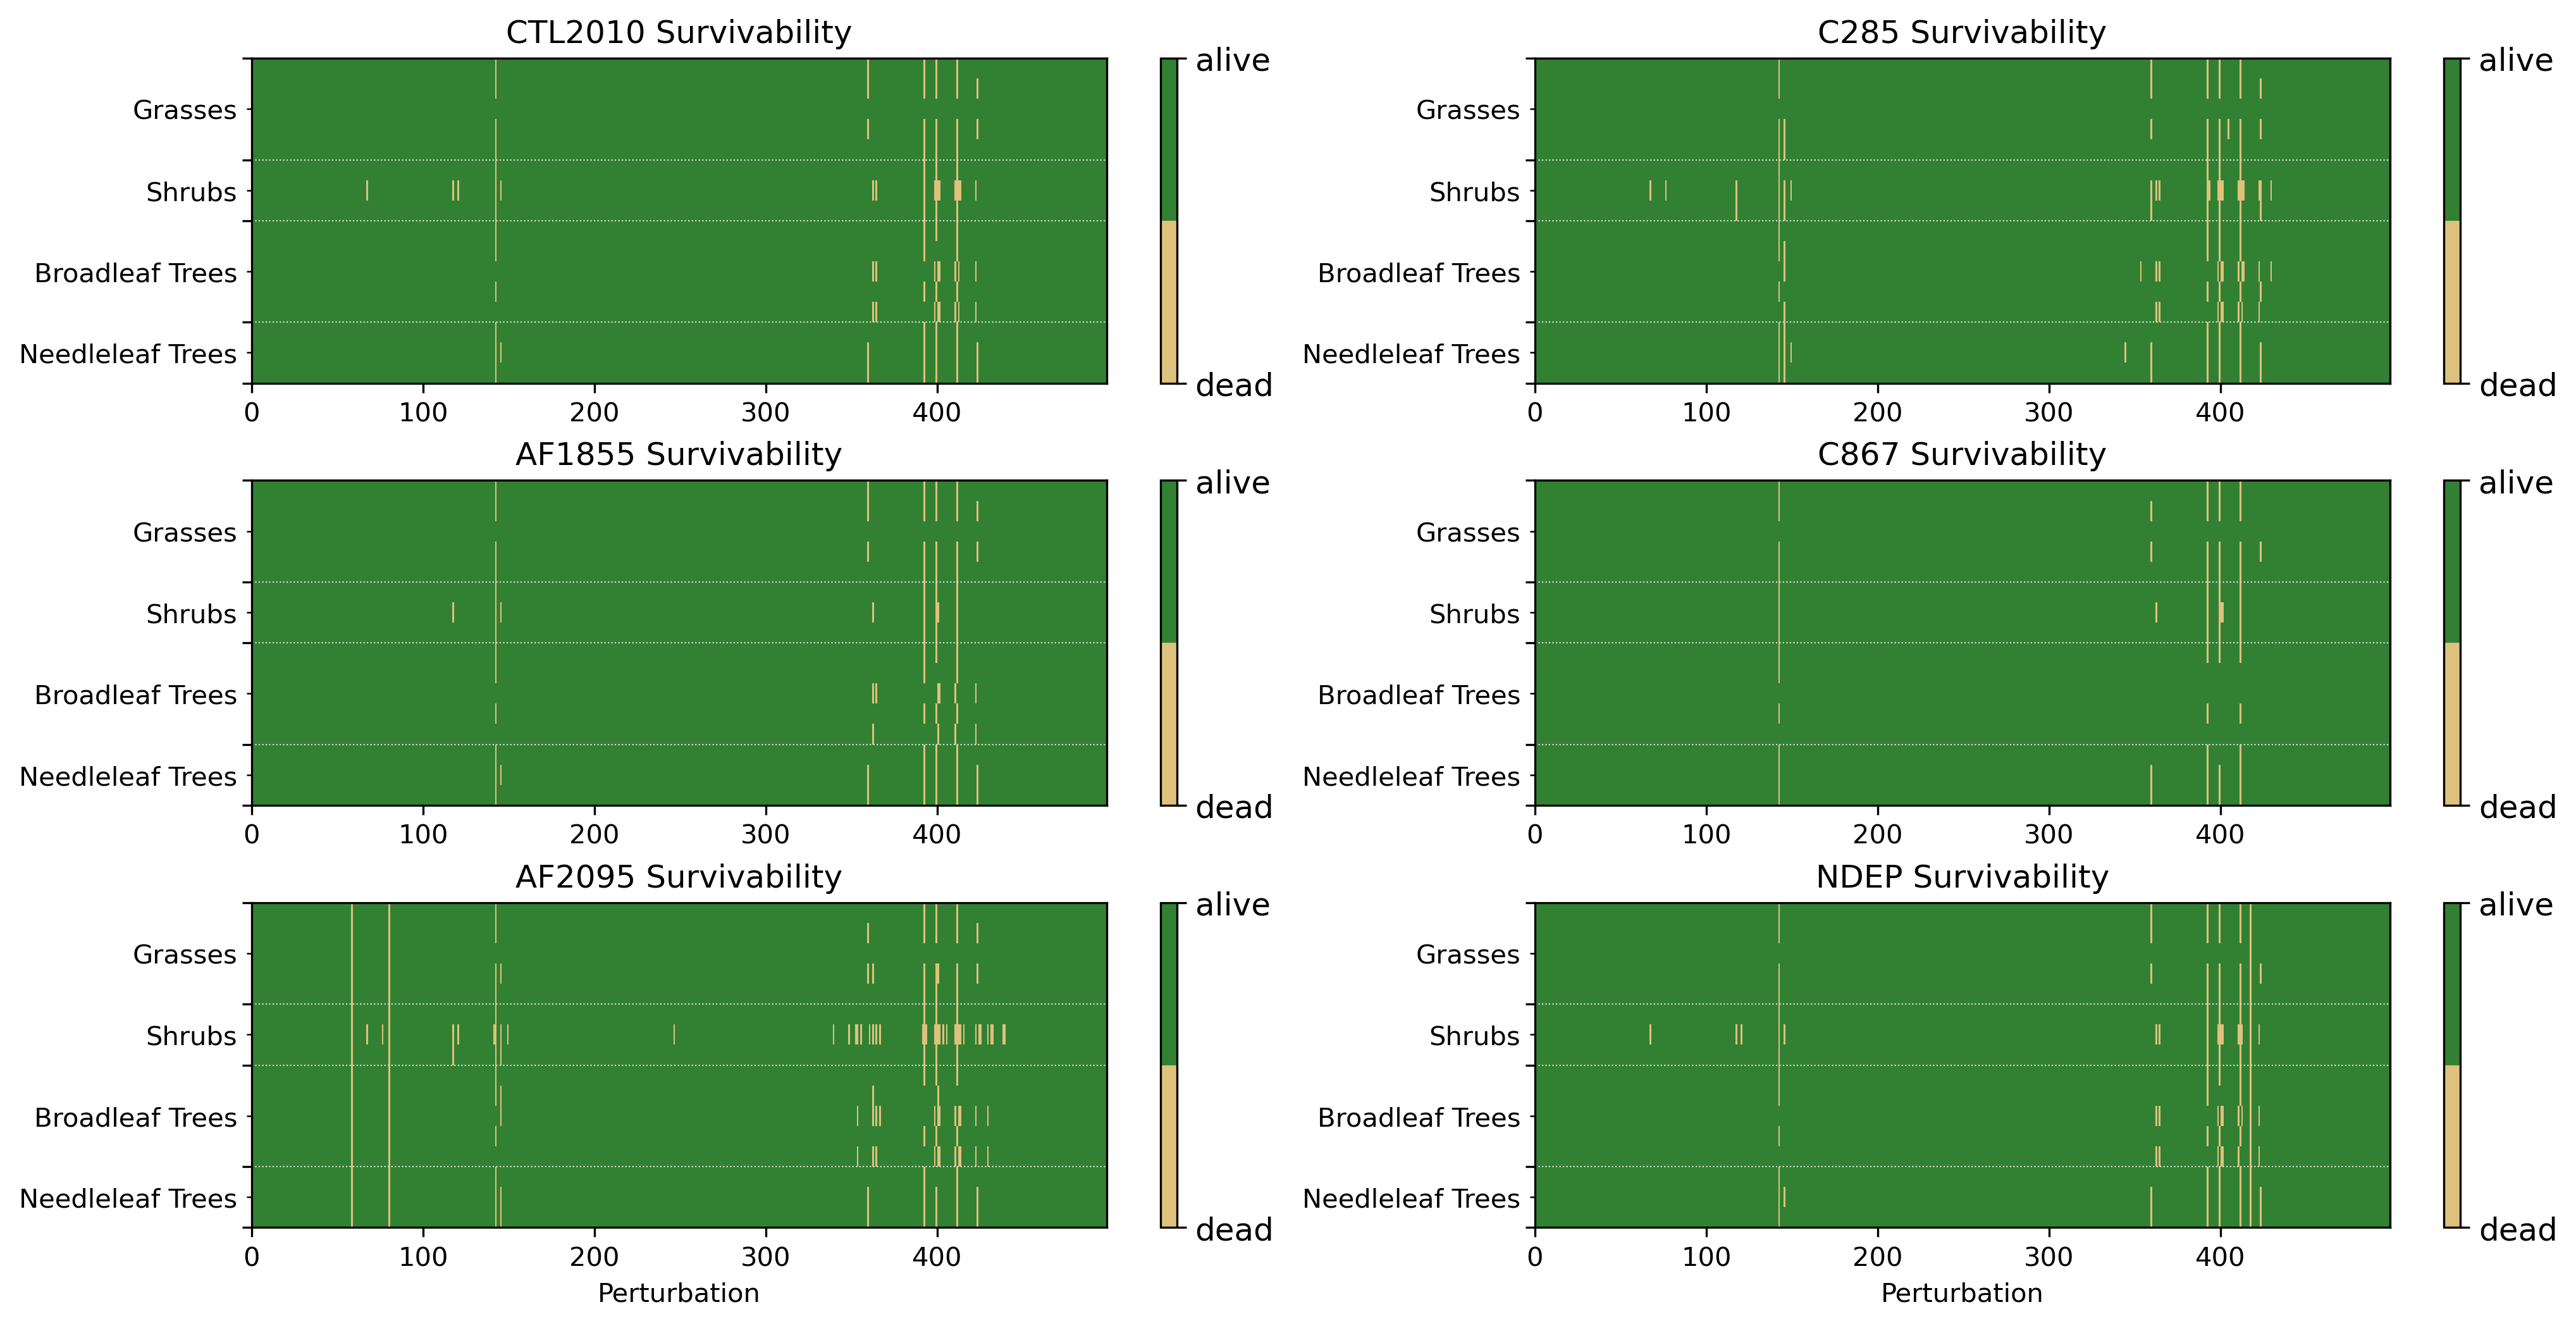
\includegraphics[width=50pc]{figs/supp/survivability.png}
\caption{PFT survivability across the six ensembles. The sixteen natural vegetation PFTs are on the vertical axis, and the perturbation number sets the horizontal axis. A PFT is classified as dead in a given gridcell if it does not achieve an LAI of at least 0.1 m2/m2 at any point during the simulation. A PFT is classified as dead for a given perturbation if more than 50\% of the area that was alive with the default parameters is dead in the perturbed simulation.}
\label{supp:surv}
\end{figure}


\begin{figure}[h]
\centering
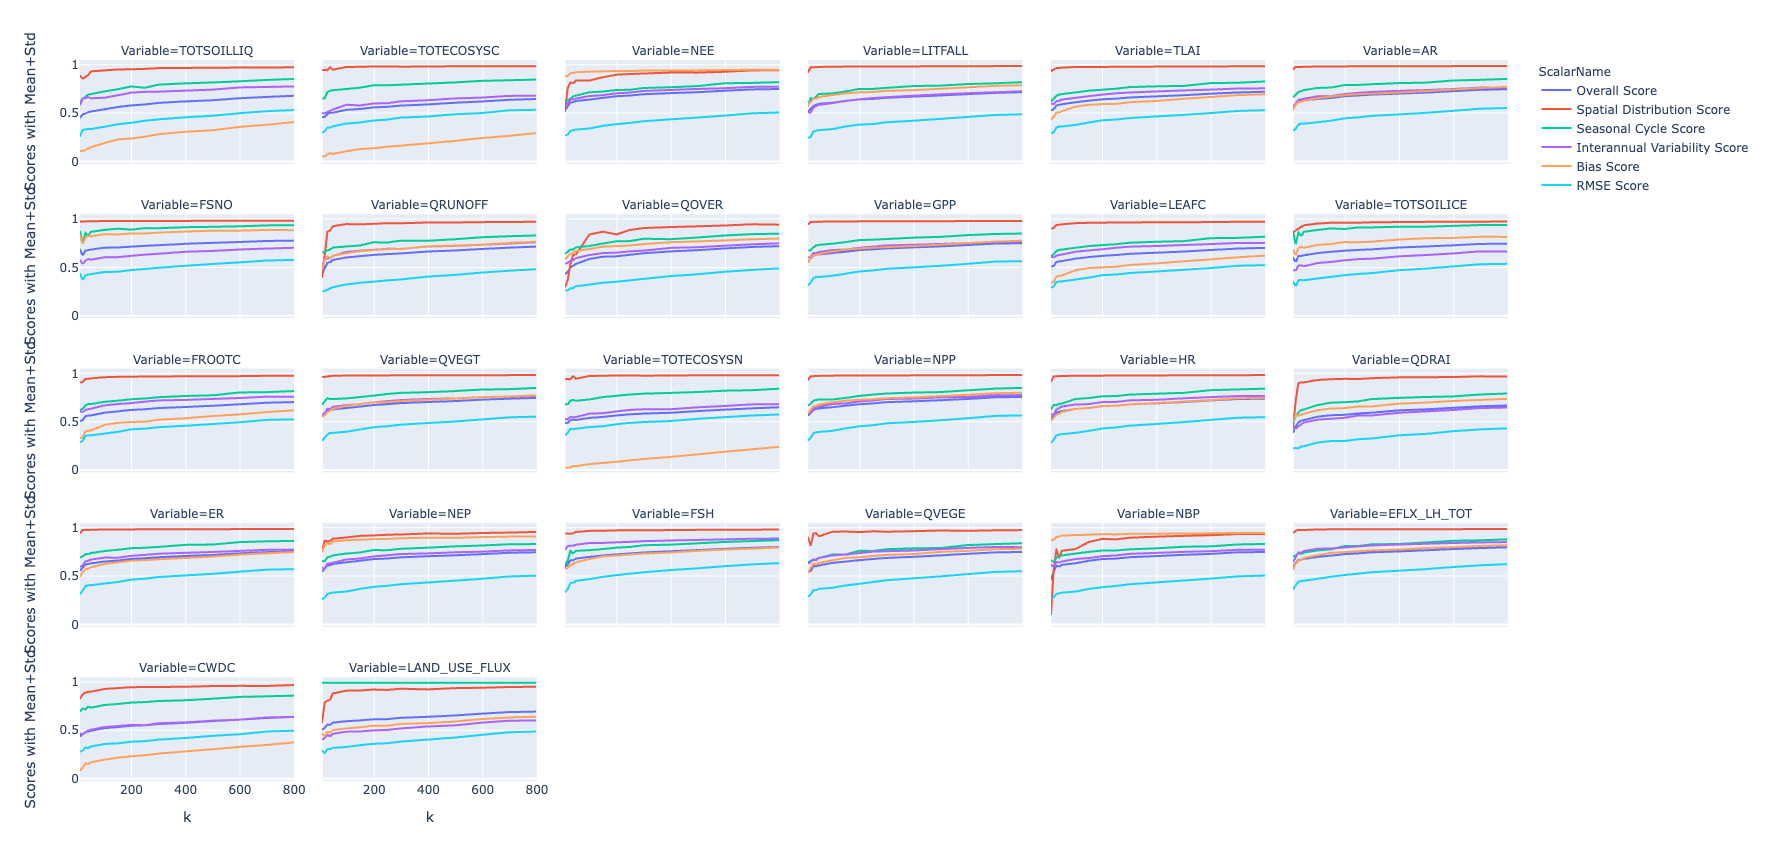
\includegraphics[width=60pc]{figs/supp/ilamb_lines.png}
\caption{The convergence of several scoring metrics with increasing sparsegrid resolution across a variety of CLM variables. All scores tend towards 1 as the number of sparsegrid clusters (k) approaches the 5666 gridcells for the native resolution of our 2-degree simulations. }
\label{supp:ilamb}
\end{figure}
\end{landscape}

\begin{figure}[h]
\centering
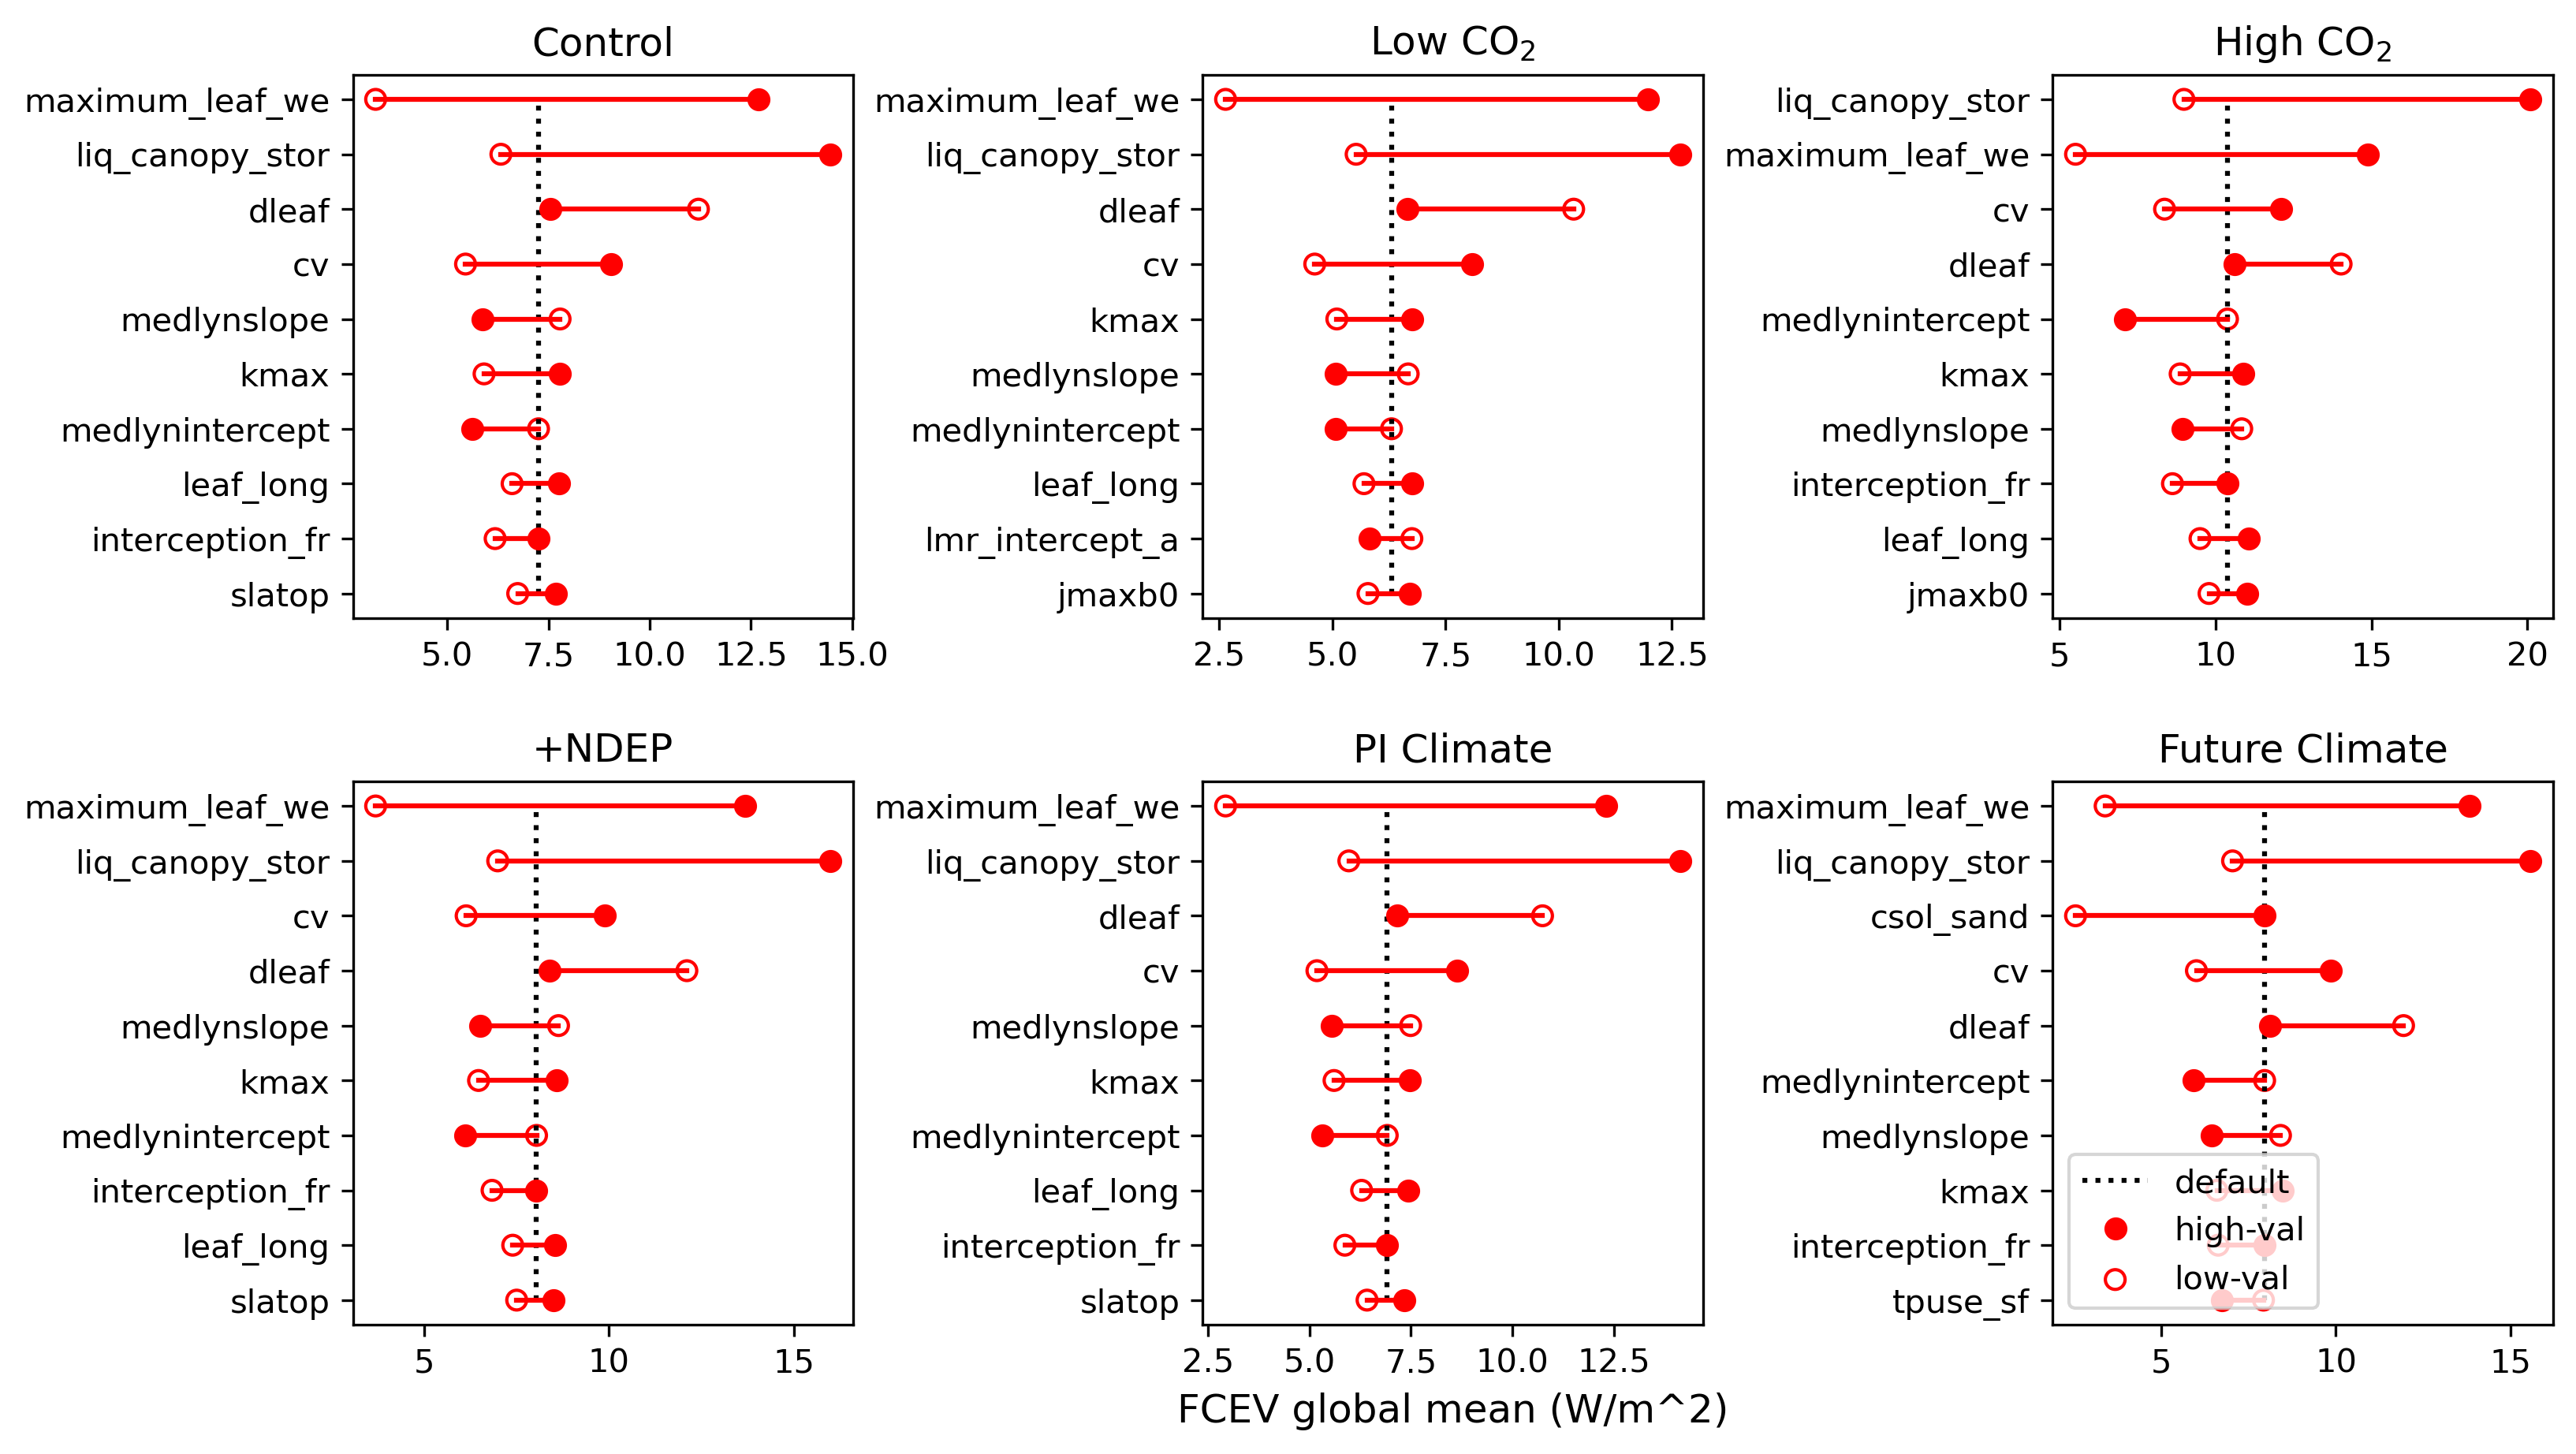
\includegraphics[width=\textwidth]{figs/supp/FCEV_global_mean.png}
\caption{Global mean canopy evaporation (FCEV) parameter rankings across the six forcing scenarios.}
\label{supp:fcev}
\end{figure}

\begin{figure}[h]
\centering
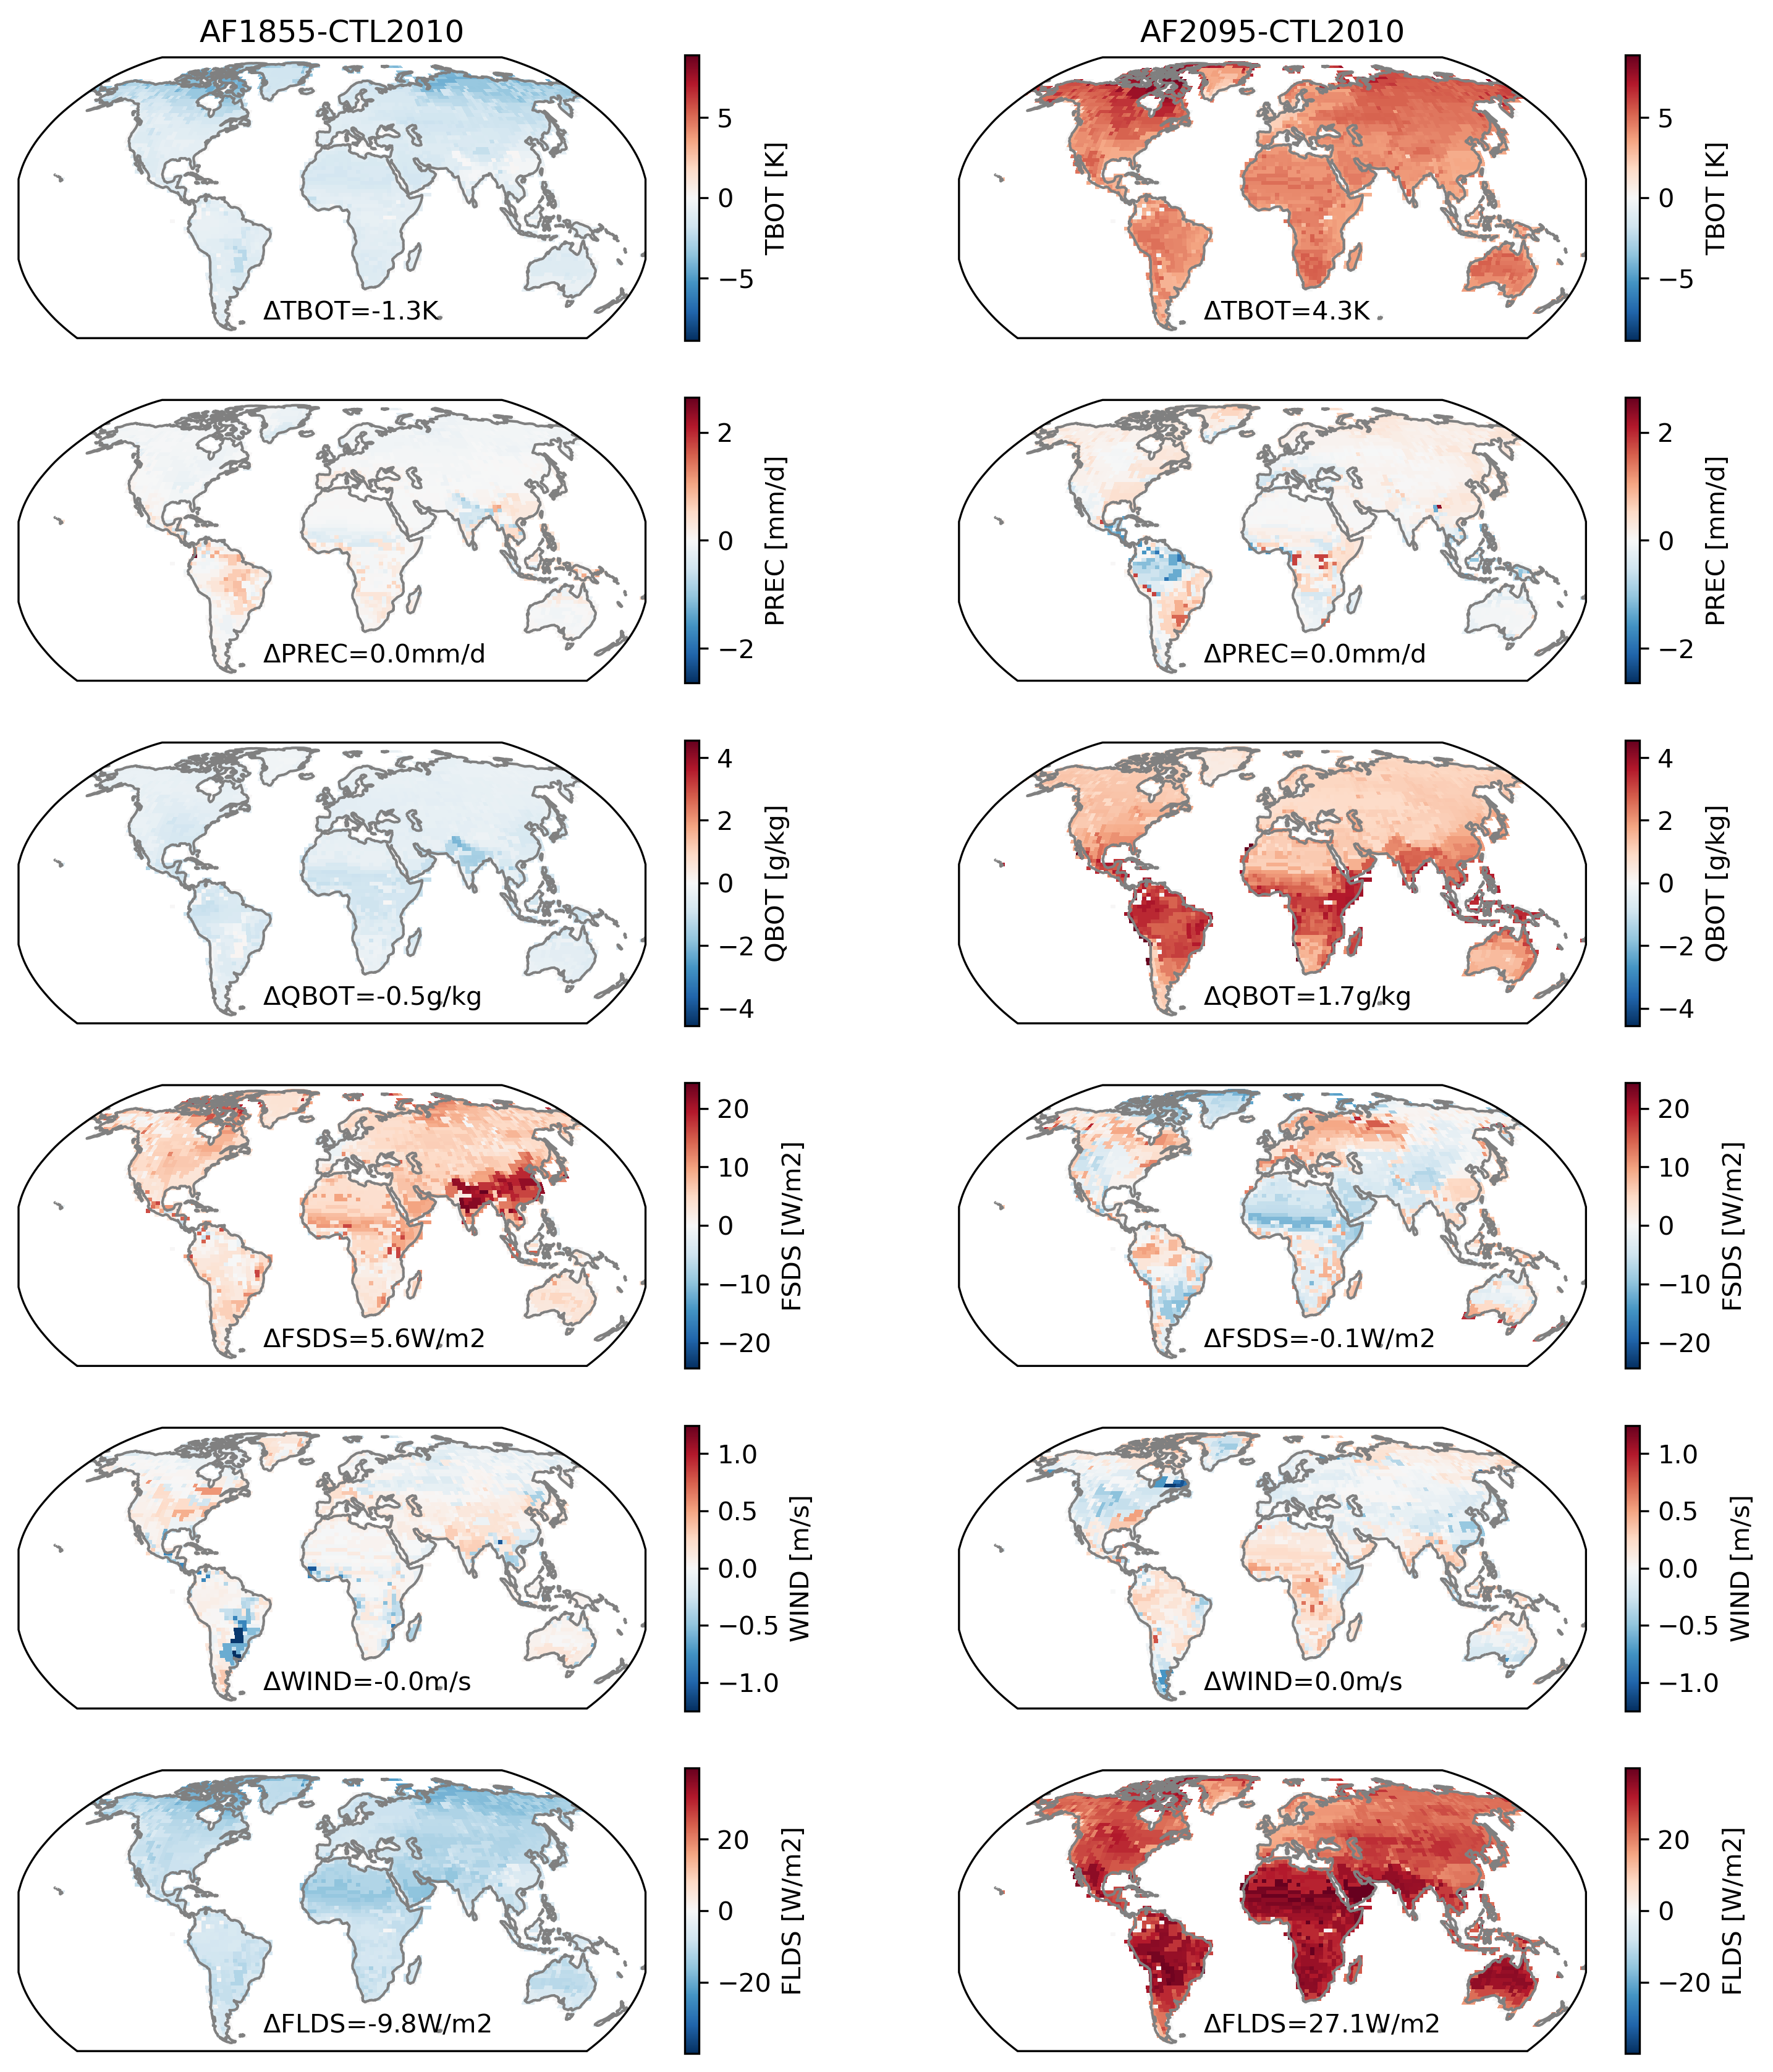
\includegraphics[width=\textwidth]{figs/supp/anomalies.png}
\caption{Maps of average forcing anomalies in the pre-industrial (left column) and future climate forcing (right column) simulations. Global averages over land, Antarctica excluded, are written in text on each subplot.}
\label{supp:anomalies}
\end{figure}

\begin{figure}[h]
\centering
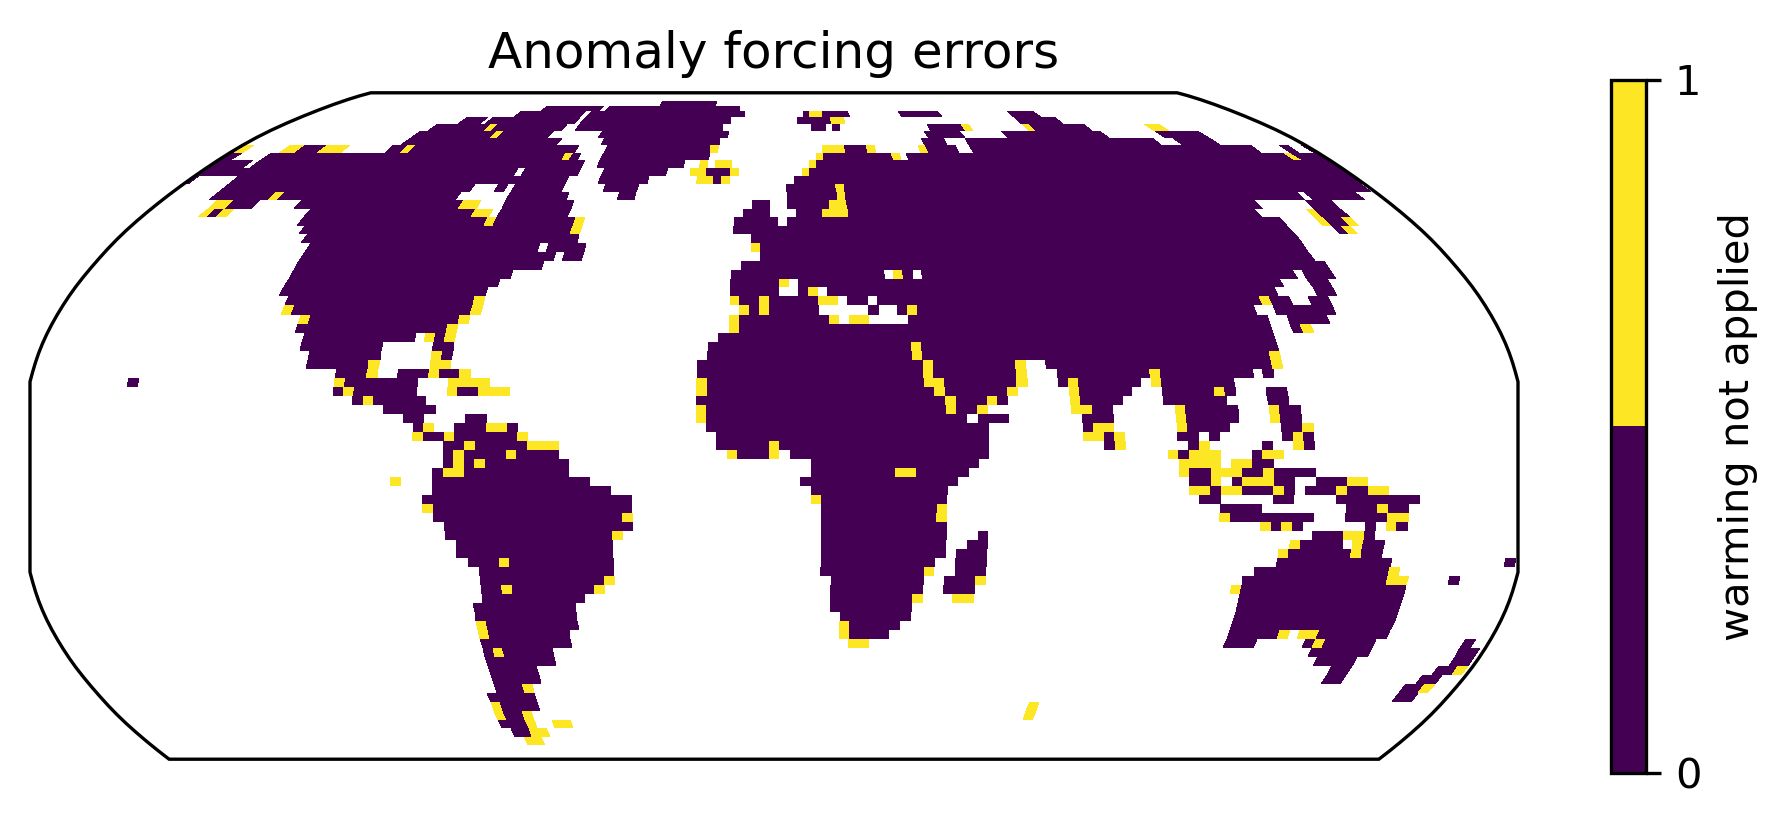
\includegraphics[width=\textwidth]{figs/supp/anomaly_errors.png}
\caption{buggy climate forcing}
\label{supp:abug}
\end{figure}

\begin{figure}[h]
\centering
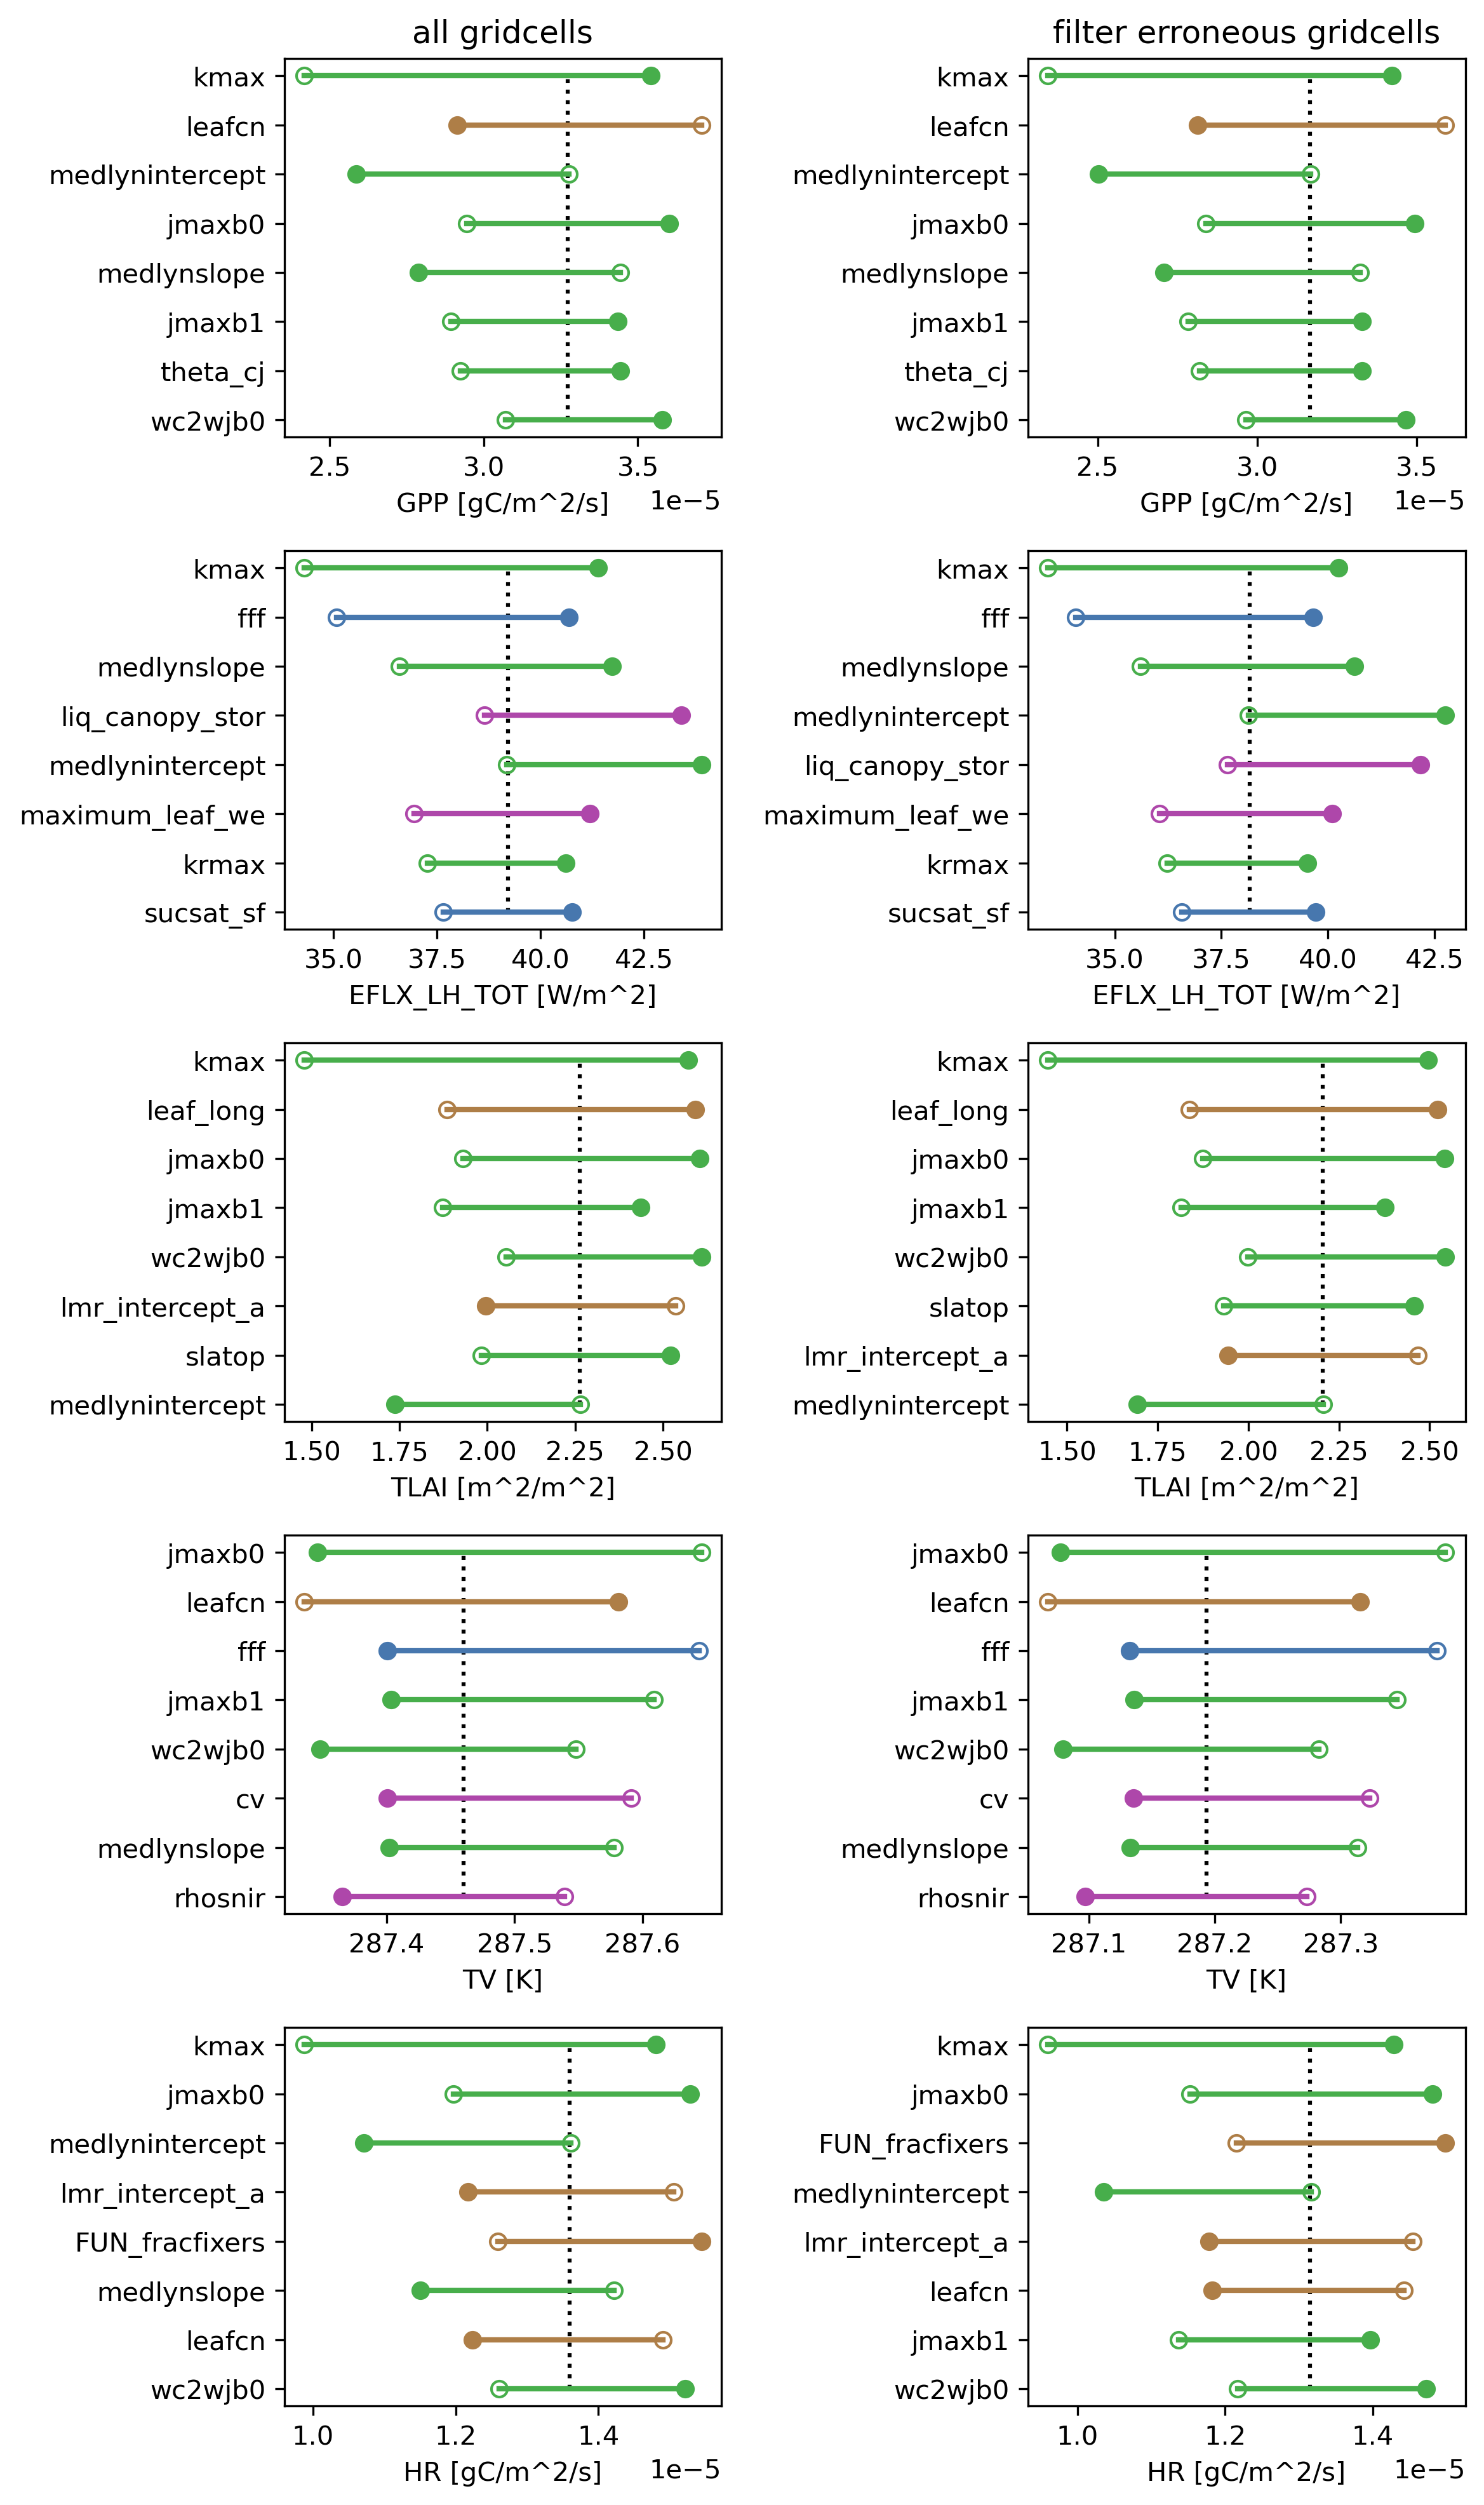
\includegraphics[width=30pc]{figs/supp/AF2095_rankings.png}
\caption{buggy climate forcing}
\label{supp:abug}
\end{figure}




\end{document}
